% Memoria del Proyecto 3 de PIDS. Se compila con `python memoria/compilar.py`
% (genera las cifras desde resultados/tablas y llama a latexmk). Ver memoria/README.md.
\documentclass[11pt,a4paper]{article}

% --- Formato de la asignatura: Calibri 11 (aquí Carlito, con las mismas métricas),
% interlineado 1,15 y márgenes de 2,5 cm.
\usepackage[T1]{fontenc}
\usepackage[sfdefault,lining]{carlito}
\usepackage[spanish,es-tabla,es-noshorthands,es-nodecimaldot]{babel}
\usepackage[a4paper,margin=2.5cm]{geometry}
\usepackage{setspace}
\setstretch{1.15}
\usepackage{microtype}
\usepackage[section]{placeins}  % las figuras no pasan a otra sección
\usepackage{float}
% Deja que las figuras compartan página con el texto en vez de ir a páginas sueltas.
\renewcommand{\topfraction}{0.85}\renewcommand{\bottomfraction}{0.6}
\renewcommand{\textfraction}{0.1}\renewcommand{\floatpagefraction}{0.8}
\setcounter{topnumber}{3}\setcounter{totalnumber}{4}
\usepackage{graphicx}
\usepackage{booktabs,tabularx,array,makecell}
\usepackage[table]{xcolor}
\usepackage{enumitem}
\usepackage[font=small,labelfont=bf,labelsep=period]{caption}
\usepackage{csquotes}
\usepackage[style=ieee,backend=biber,doi=true,url=true,dashed=false]{biblatex}
\addbibresource{referencias.bib}
\DefineBibliographyStrings{spanish}{url={Disponible en}}
\usepackage[hidelinks]{hyperref}

\setlist{itemsep=1pt,topsep=3pt}
\setlength{\parskip}{4pt}
\setlength{\parindent}{0pt}
\graphicspath{{../resultados/figuras/exploracion/}{../resultados/figuras/movilidad/}}
\definecolor{tenue}{HTML}{526576}
\definecolor{fondo}{HTML}{F2F5F8}
\newcolumntype{Y}{>{\raggedright\arraybackslash}X}

% --- Cifras: las escribe memoria/generar_cifras.py desde resultados/tablas.
\newcommand\defcifra[2]{\expandafter\def\csname cifra@#1\endcsname{#2}}
\newcommand\cifra[1]{\ifcsname cifra@#1\endcsname\csname cifra@#1\endcsname
  \else\PackageError{memoria}{Cifra desconocida: \detokenize{#1}}{Revisa generar_cifras.py}\fi}
% Generado por memoria/generar_cifras.py a partir de resultados/tablas. No editar a mano.
\defcifra{arista_res8_m}{531}
\defcifra{arista_res9_m}{201}
\defcifra{asig_acceso_d}{163}
\defcifra{asig_acceso_o}{162}
\defcifra{asig_acceso_p90}{264}
\defcifra{asig_acceso_pie}{215}
\defcifra{asig_asimetria}{38,4}
\defcifra{asig_asimetria_azar}{34,6}
\defcifra{asig_atendidos}{12\,750}
\defcifra{asig_circular_pct}{12,3}
\defcifra{asig_pares}{4\,090}
\defcifra{asig_pares_pct}{16,2}
\defcifra{asig_pct_total}{76,1}
\defcifra{asig_rechazos}{659}
\defcifra{asig_rechazos_top10}{17,5}
\defcifra{asig_spearman}{\textminus{}0,40}
\defcifra{asig_top10_pct}{4,0}
\defcifra{autonomia_mediana_dias}{45,3}
\defcifra{caida_21_pct}{30}
\defcifra{caida_22_pct}{60}
\defcifra{candidatos_avisos}{65}
\defcifra{candidatos_desplazados}{7}
\defcifra{candidatos_n}{600}
\defcifra{celda_kwh_max}{0,90}
\defcifra{celda_kwh_p50}{0,13}
\defcifra{celdas_emisoras}{42}
\defcifra{celdas_receptoras}{45}
\defcifra{celdas_res8}{111}
\defcifra{celdas_res9}{600}
\defcifra{celdas_res9_80}{226}
\defcifra{celdas_res9_95}{381}
\defcifra{celdas_saldo}{90}
\defcifra{cierre_anc}{966}
\defcifra{cierre_atendidos_aj}{12\,750}
\defcifra{cierre_atendidos_res}{4\,670}
\defcifra{cierre_bat_pendiente}{0,067}
\defcifra{cierre_bat_rechazos}{0}
\defcifra{cierre_equidad_pp}{6,31}
\defcifra{cierre_extra_reb}{4}
\defcifra{cierre_fallos_habitual}{48}
\defcifra{cierre_fallos_redundante}{48}
\defcifra{cierre_km_ahorro}{75,9}
\defcifra{cierre_km_ajuste}{2\,416,8}
\defcifra{cierre_kw_est}{0,48}
\defcifra{cierre_kw_red}{3,46}
\defcifra{cierre_kwh_dia_aj}{16,64}
\defcifra{cierre_kwh_dia_res}{18,76}
\defcifra{cierre_pct_cub_res}{93,38}
\defcifra{cierre_pct_total_res}{70,61}
\defcifra{cierre_solicitudes_res}{6\,614}
\defcifra{cierre_top10}{16,82}
\defcifra{cierre_zonas}{8}
\defcifra{circulares_pct}{3,59}
\defcifra{cociente_lluvia}{69}
\defcifra{cociente_lluvia_finde}{48}
\defcifra{cociente_lluvia_lab}{88}
\defcifra{concentracion_20pc_res8}{56,9}
\defcifra{concentracion_20pc_res9}{58,1}
\defcifra{consumo_wh_km}{13,5}
\defcifra{desfase_0}{30,8}
\defcifra{desfase_mas1}{31,0}
\defcifra{dias_lluvia}{6}
\defcifra{diferencia_perfiles_pct}{12,0}
\defcifra{dis_mediana_m}{1\,619}
\defcifra{enc_cob_ajuste}{80,22}
\defcifra{enc_pares}{1\,045}
\defcifra{enc_pct}{4,47}
\defcifra{enc_ref_sigue}{20,3}
\defcifra{enc_ref_vuelve}{55,5}
\defcifra{enc_sigue}{28,7}
\defcifra{enc_vuelve}{47,3}
\defcifra{encadenamientos}{22\,855}
\defcifra{energia_sol_pct}{33,5}
\defcifra{energia_tarde_pct}{55,5}
\defcifra{entregas_red_pct}{90,3}
\defcifra{entregas_top20}{25,4}
\defcifra{estabilidad_res8}{0,98}
\defcifra{estabilidad_res9}{0,92}
\defcifra{excluidos_umbral}{1\,816}
\defcifra{fisico_central}{7,0}
\defcifra{fisico_crucero}{9,0}
\defcifra{fisico_max}{11,8}
\defcifra{flota_700_anclaje}{1\,632}
\defcifra{flota_700_pct}{87,7}
\defcifra{flota_antes}{375}
\defcifra{flota_antes_pct}{94,5}
\defcifra{flota_cargas_dia}{38,4}
\defcifra{flota_kwh_dia}{22,1}
\defcifra{flota_kwh_dia_max}{29,6}
\defcifra{flota_kwh_dia_reservada}{27,2}
\defcifra{flota_max}{475}
\defcifra{flota_max_pct}{95,9}
\defcifra{flota_min}{400}
\defcifra{flota_min_anclaje}{187}
\defcifra{flota_min_pct}{95,1}
\defcifra{flota_res_diseno}{94,2}
\defcifra{flota_res_min}{93,4}
\defcifra{flota_sin_reb_pct}{85,7}
\defcifra{flota_vpd_max}{1,29}
\defcifra{flota_vpd_min}{1,52}
\defcifra{grupo}{05}
\defcifra{inv_anclajes}{966}
\defcifra{inv_anclajes_max}{11}
\defcifra{inv_anclajes_mediana}{6}
\defcifra{inv_cuantil}{P90}
\defcifra{inv_desvio_m}{85}
\defcifra{inv_desvios}{298}
\defcifra{inv_flota}{400}
\defcifra{inv_flota_diseno}{474}
\defcifra{inv_mes_anclajes}{3\,123}
\defcifra{inv_mes_flota}{1\,556}
\defcifra{inv_noches}{20}
\defcifra{inv_noches_agotadas}{16}
\defcifra{inv_objetivo}{95}
\defcifra{inv_pct}{95,1}
\defcifra{inv_pct_anterior}{94,2}
\defcifra{inv_pct_diseno}{95,9}
\defcifra{inv_reb_max}{220}
\defcifra{inv_reb_max_pct}{96,6}
\defcifra{inv_reservada_pct}{93,4}
\defcifra{inv_sin_anclaje}{187}
\defcifra{inv_sin_desvio_pct}{93,0}
\defcifra{inv_sin_patinete}{472}
\defcifra{inv_sin_reb_max_pct}{90,1}
\defcifra{inv_vpd}{1,52}
\defcifra{km_ajuste}{34\,431}
\defcifra{lluvia_0702}{24,6}
\defcifra{lluvia_ajuste_mm}{75,7}
\defcifra{noche_pct}{2,5}
\defcifra{od_adm_asignados}{23\,346}
\defcifra{od_adm_sin_zona}{24}
\defcifra{od_asimetria}{1,09}
\defcifra{od_asimetria_azar_pct}{20,4}
\defcifra{od_asimetria_obs_pct}{22,3}
\defcifra{od_h3_intra_muestra_adm_pct}{21,2}
\defcifra{od_interzonales_ajuste}{13\,168}
\defcifra{od_intrazonales_pct}{21,4}
\defcifra{od_manana_fds_dia}{34,5}
\defcifra{od_manana_lab_dia}{114,7}
\defcifra{od_matrices_temporales}{90}
\defcifra{od_municipio_intra_pct}{73,6}
\defcifra{od_pares}{2\,157}
\defcifra{od_top10_inter_pct}{10,6}
\defcifra{od_top20_pct}{14,8}
\defcifra{od_top30_pct}{51,0}
\defcifra{od_urbanistica_intra_pct}{41,8}
\defcifra{oferta_vacia_max}{26,5}
\defcifra{oferta_vacia_mediana}{5,7}
\defcifra{operador_compensado_pct}{62,1}
\defcifra{operador_pendiente}{0,75}
\defcifra{operador_spearman}{0,89}
\defcifra{origenes_red_pct}{89,9}
\defcifra{paradas_dis_min_m}{1\,000}
\defcifra{paradas_fuera}{52}
\defcifra{paradas_fuera_tt_h}{4,4}
\defcifra{paradas_largos}{10}
\defcifra{paradas_lentos}{68}
\defcifra{paradas_lentos_dis}{1\,636}
\defcifra{paradas_lentos_recta}{782}
\defcifra{paradas_lentos_tt}{91}
\defcifra{paradas_tt_max_h}{2,5}
\defcifra{paradas_viajes}{78}
\defcifra{parado_recolocado_h}{98,8}
\defcifra{parado_sin_salto_h}{5,8}
\defcifra{pares_azar}{21,9}
\defcifra{pares_semanas_max}{7,6}
\defcifra{pares_semanas_min}{4,7}
\defcifra{pares_tvd}{27,4}
\defcifra{patinetes}{2\,331}
\defcifra{patinetes_activos_dia}{487,8}
\defcifra{patinetes_elegibles}{2\,305}
\defcifra{patinetes_recolocados}{2\,094}
\defcifra{pct_elegibles}{92,8}
\defcifra{pct_mediana_0702}{46,6}
\defcifra{pendiente_ajuste}{9,4}
\defcifra{pendiente_mes}{10,6}
\defcifra{pendiente_mes_tiempo}{7,6}
\defcifra{permisiva_mas_pct}{2,5}
\defcifra{punta_manana_finde_pct}{4,4}
\defcifra{punta_manana_lab_pct}{14,4}
\defcifra{punta_tarde_finde_pct}{43,2}
\defcifra{punta_tarde_lab_pct}{38,0}
\defcifra{rebalanceo_base}{100}
\defcifra{rebalanceo_estructural_res8}{42,9}
\defcifra{rebalanceo_res8}{101,5}
\defcifra{rebalanceo_res8_max}{138}
\defcifra{rebalanceo_res9}{221,6}
\defcifra{rebalanceo_sensibilidad}{0 y 220}
\defcifra{recogidas_top20}{13,9}
\defcifra{recolocacion_km}{3,67}
\defcifra{recolocaciones}{5\,111}
\defcifra{recolocaciones_dia}{182,5}
\defcifra{recolocaciones_intradia_pct}{0,9}
\defcifra{recolocaciones_noche_pct}{98,8}
\defcifra{red_ajuste_comparables}{969}
\defcifra{red_ajuste_geo_pct}{80,03}
\defcifra{red_ajuste_linea_pct}{86,0}
\defcifra{red_ajuste_pie_delta}{\textminus{}41,5}
\defcifra{red_ajuste_pie_pct}{44,5}
\defcifra{red_ajuste_ruta_p90}{413}
\defcifra{red_alternativa_k}{158}
\defcifra{red_alternativa_pct}{79,79}
\defcifra{red_estaciones}{159}
\defcifra{red_lscp_cota}{154}
\defcifra{red_lscp_factible}{159}
\defcifra{red_lscp_margen}{4}
\defcifra{red_mclp_brecha}{194}
\defcifra{red_mclp_ganancia}{179}
\defcifra{red_peor_dia}{26/02}
\defcifra{red_peor_pct}{72,94}
\defcifra{red_peor_viajes}{1\,094}
\defcifra{red_pie_sensibilidad_pct}{78,2}
\defcifra{red_pie_umbral_max}{400}
\defcifra{red_pierde_ambos}{81}
\defcifra{red_pierde_d}{172}
\defcifra{red_pierde_o}{149}
\defcifra{red_radio}{300}
\defcifra{red_radio_menor}{250}
\defcifra{red_radio_menor_k}{225}
\defcifra{red_reservada_comparables}{431}
\defcifra{red_reservada_geo_pct}{75,61}
\defcifra{red_reservada_linea_pct}{82,4}
\defcifra{red_reservada_pie_delta}{\textminus{}38,1}
\defcifra{red_reservada_pie_pct}{44,3}
\defcifra{red_reservada_ruta_p90}{422}
\defcifra{red_variacion_dentro}{\textminus{}4,38}
\defcifra{red_variacion_geo}{\textminus{}4,41}
\defcifra{red_variacion_mezcla}{\textminus{}0,03}
\defcifra{redes_base_eval_n}{166}
\defcifra{redes_base_k_max_300}{207}
\defcifra{redes_base_k_ref}{141}
\defcifra{redes_base_means_ref_pct}{58,4}
\defcifra{redes_base_medoids_ref_pct}{60,8}
\defcifra{redes_base_mejor_max_pct}{75,9}
\defcifra{redes_base_n}{118}
\defcifra{reservada_mas_pct}{18,4}
\defcifra{resto_dis}{1\,634}
\defcifra{resto_tt}{8,2}
\defcifra{rho_lluvia}{\textminus{}0,56}
\defcifra{rho_lluvia_finde}{\textminus{}0,46}
\defcifra{rho_lluvia_parcial_finde}{\textminus{}0,29}
\defcifra{rho_viento_finde}{\textminus{}0,88}
\defcifra{rho_viento_lluvia_finde}{0,38}
\defcifra{rho_viento_parcial_finde}{\textminus{}0,86}
\defcifra{rodeo}{1,329}
\defcifra{salto_mediana_m}{16,9}
\defcifra{simultaneos_max}{41}
\defcifra{tarifa_desbloqueo}{1}
\defcifra{tarifa_discrepancias}{0}
\defcifra{tarifa_importe_elegible}{63\,205,67}
\defcifra{tarifa_importe_excluido_pct}{17,3}
\defcifra{tarifa_importe_largos}{10\,335,96}
\defcifra{tarifa_minuto}{0,15}
\defcifra{temp_ajuste}{9,3}
\defcifra{temp_reservada}{10,9}
\defcifra{tt_mediana_min}{8,2}
\defcifra{vel_mediana}{12,5}
\defcifra{velocidad_pie}{1,3}
\defcifra{viajes_0702}{403}
\defcifra{viajes_1402}{721}
\defcifra{viajes_ajuste}{16\,756}
\defcifra{viajes_brutos}{25\,186}
\defcifra{viajes_dia_ajuste}{797,9}
\defcifra{viajes_dia_finde}{793,5}
\defcifra{viajes_dia_laborable}{799,7}
\defcifra{viajes_dia_reservada}{944,9}
\defcifra{viajes_elegibles}{23\,370}
\defcifra{viajes_reservada}{6\,614}
\defcifra{viento_finde_inf}{\textminus{}23}
\defcifra{viento_finde_pct}{14}
\defcifra{viento_finde_sup}{\textminus{}5}
\defcifra{viento_lab_pct}{7}
\defcifra{viento_max_ajuste}{18,3}
\defcifra{viento_max_reservada}{13,5}
\defcifra{viento_secas_finde}{76}

\newcommand\pc{\,\%}
% Ruta de un notebook o tabla del repositorio: se escribe tal cual y puede cortarse en / y _.
\DeclareUrlCommand\nb{\urlstyle{tt}}
\def\UrlBreaks{\do\/\do\_\do\.}
\setcounter{biburlnumpenalty}{100}\setcounter{biburlucpenalty}{100}\setcounter{biburllcpenalty}{100}
\newcommand\fechaversion{18/11/2026}

\title{Red de estaciones de recarga para patinetes eléctricos compartidos en Roma}
\author{Alejandro Cuevas \and Javier Saguar}
\date{\fechaversion}

\begin{document}

% ------------------------------------------------------------------------------------------
\begin{titlepage}
  \centering
  {\large UNIVERSIDAD POLITÉCNICA DE MADRID\par}
  {Escuela Técnica Superior de Ingenieros de Telecomunicación\par}
  \vspace{1.2cm}
  {\large Proyectos en Ingeniería de Datos y Sistemas (PIDS)\par}
  {Proyecto 3\par}
  \vspace{2.2cm}
  {\LARGE\bfseries Red de estaciones de recarga para patinetes\\[2pt] eléctricos compartidos en Roma\par}
  \vspace{0.6cm}
  {\large MEMORIA DEL PROYECTO\par}
  \vfill
  \renewcommand{\arraystretch}{1.4}
  \begin{tabular}{@{}r@{\hspace{1.2em}}l@{}}
    \textbf{Grupo} & G\cifra{grupo} \\
    \textbf{Autores} & Cuevas, Alejandro \\
                     & Saguar, Javier \\
    \textbf{Versión} & Fase 0 completa y comienzo de la fase 1 \\
    \textbf{Fecha} & \fechaversion \\
    \textbf{Curso académico} & 2026/2027 \\
  \end{tabular}
  \vspace{2cm}
\end{titlepage}

% ------------------------------------------------------------------------------------------
\section*{Reparto del trabajo}
\addcontentsline{toc}{section}{Reparto del trabajo}

\begin{table}[h]
  \centering\small
  \caption{Reparto del trabajo hasta esta versión. Las tareas están en \texttt{docs/TAREAS.md} \cite{codigo}.}
  \begin{tabularx}{\textwidth}{@{}lYY@{}}
    \toprule
    Integrante & Fase 0: datos y exploración & Fase 1: movilidad \\
    \midrule
    Javier Saguar (líder) & Entorno reproducible, paquete \nb{comun/} y \nb{config.yaml}; limpieza (T10), recolocaciones (T11), patrones temporales (T12); web de resultados; viento frente a lluvia (T17, apartado 6); esta memoria & Revisión de T20 y decisiones de la fase \\
    \addlinespace
    Alejandro Cuevas & Densidad en H3 (T13), saldo por celda (T14), recorridos y radios (T15), energía de referencia (T16), meteorología (T17) & Primera matriz O-D en H3 (T20) \\
    \bottomrule
  \end{tabularx}
\end{table}

\section*{Estado de esta versión}
\addcontentsline{toc}{section}{Estado de esta versión}
La memoria se escribe a la vez que el proyecto. Esta versión recoge la fase~0 completa
(limpieza y exploración, que fija los parámetros de las demás fases) y la primera matriz
origen-destino de la fase~1. De los apartados de movilidad, consumo y estación de recarga
se describe el método previsto y lo que ya fija la exploración; sus resultados entrarán en
las versiones siguientes.

\newpage
\tableofcontents
\newpage

% ------------------------------------------------------------------------------------------
\section{Introducción}

\subsection{Problema}
Una empresa quiere implantar en Roma un servicio de patinetes eléctricos compartidos. El
Ayuntamiento exige que, cuando no se usen, los patinetes queden anclados en estaciones de
recarga y no en la acera. A partir de los viajes de un piloto de Helbiz en febrero de 2021
\cite{datos} hay que decidir cuántas estaciones poner, dónde, con cuántos anclajes y
patinetes, cuánta energía consume la flota y cómo alimentar una estación concreta con
paneles fotovoltaicos y baterías \cite{enunciado}.

Los objetivos chocan entre sí. Menos estaciones con más patinetes cada una obligan a andar
más desde el origen y hasta el destino de cada viaje. Una flota pequeña y muy usada deja
estaciones vacías en las horas punta. La solución es un compromiso, y esta memoria justifica
cada elección con cifras.

\subsection{Enfoque}
\begin{itemize}
  \item \textbf{Exploración orientada a decisiones.} Cada análisis de la fase~0 responde a una
        pregunta y fija un parámetro de las fases siguientes: umbrales de limpieza, franjas
        horarias, rejilla de candidatos, radios de acceso, rebalanceo y días de diseño.
  \item \textbf{Validación temporal.} Los parámetros se ajustan con los viajes del 1 al 21 de
        febrero (periodo de \emph{ajuste}). La semana del 22 al 28 (\emph{reservada}) solo
        se usa para validar la red.
  \item \textbf{Reproducibilidad.} Todo se regenera desde el CSV original con un único
        script, \nb{ejecutar_todo.py}, y los parámetros están en \nb{config.yaml}
        \cite{codigo}. Las cifras de esta memoria no se escriben a mano: un script las lee
        de las tablas de resultados (apartado~\ref{sec:reproducibilidad}).
\end{itemize}

% ------------------------------------------------------------------------------------------
\section{Datos y método}

\subsection{Datos de partida}
El fichero tiene \cifra{viajes_brutos} viajes de \cifra{patinetes} patinetes con
identificador, hora de salida y de llegada, precio, duración, distancia recorrida,
velocidad media y coordenadas de origen y destino \cite{datos}. El enunciado menciona
trayectorias con un punto cada 10~s, pero el fichero no las incluye: solo se conocen los
extremos de cada viaje. El precio es exactamente 1~€ más 0,15~€ por minuto y la
distancia es la del recorrido, no la línea recta. Los datos meteorológicos son de la API
histórica de Open-Meteo para Roma centro \cite{openmeteo,era5}.

\subsection{Reproducibilidad}\label{sec:reproducibilidad}
El repositorio \cite{codigo} separa los datos originales, que no se modifican nunca, de los
derivados. El paquete \nb{comun/} carga los viajes limpios y los regenera si cambian los
umbrales de \nb{config.yaml}. Cada tarea es un notebook con su objetivo, un bloque por
análisis (qué se quiere ver, por qué importa, código y conclusiones) y una tabla de
decisiones. \nb{ejecutar_todo.py} los ejecuta en orden y guarda tablas, figuras y los
datos de la web de resultados \cite{web}. Las respuestas de servicios externos se guardan
con su fecha y su fuente para poder reproducir sin conexión. Las cifras de esta memoria
salen de \nb{memoria/generar_cifras.py}, que lee \nb{resultados/tablas/}. Se han usado
pandas \cite{pandas}, SciPy \cite{scipy}, Matplotlib \cite{matplotlib} y H3 \cite{h3}.

\subsection{Limpieza}
No hay nulos, duplicados, solapes del mismo patinete ni extremos fuera de Roma, y la
duración, la velocidad y el precio cuadran en todos los viajes
(\nb{exploracion/T10_limpieza.ipynb} \cite{codigo}). Por eso solo se excluyen viajes por
umbrales de comportamiento (tabla~\ref{tab:embudo}). Ningún viaje se borra: cada uno lleva
el motivo de su exclusión. Quedan \textbf{\cifra{viajes_elegibles} viajes elegibles}
(\cifra{pct_elegibles}\pc): \cifra{viajes_ajuste} en el ajuste y \cifra{viajes_reservada}
en la semana reservada.

\begin{table}[htb]
  \centering\small
  \caption{Embudo de limpieza. Las reglas se aplican en este orden.}\label{tab:embudo}
  \begin{tabular}{@{}lrr@{}}
    \toprule
    Regla & Excluidos & Quedan \\
    \midrule
    % Generado por memoria/generar_cifras.py. No editar a mano.
Viajes del fichero original & & 25\,186 \\
Nulos, duplicados, incoherencias, fuera de zona y solapes & 0 & 25\,186 \\
Duración mayor de 2 h (\texttt{tt\_largo}) & 122 & 25\,064 \\
Velocidad mayor de 25 km/h (\texttt{vel\_alta}) & 2 & 25\,062 \\
Duración menor de 60 s (\texttt{tt\_corto}) & 949 & 24\,113 \\
Distancia menor de 100 m (\texttt{dis\_corta}) & 596 & 23\,517 \\
Velocidad menor de 2 km/h (\texttt{vel\_baja}) & 225 & 23\,292 \\
\bottomrule
% termina en \bottomrule
  \end{tabular}
\end{table}

Los umbrales salen de los histogramas (figura~\ref{fig:umbrales}). El pico de casi mil viajes
a 0~km/h son desbloqueos sin viaje, que ya quitan la duración y la distancia mínimas. La
regla de 2~km/h quita viajes de distancia normal pero muy largos: patinetes que no se
cerraron o que se llevaron a mano. Una limpieza más permisiva (30~s, 50~m, sin velocidad
mínima, 30~km/h y 3~h) deja un \cifra{permisiva_mas_pct}\pc{} más de viajes y no cambia los
indicadores clave: las medianas varían menos de un 3\pc{} y la concentración espacial
(\cifra{concentracion_20pc_res8}\pc{} de los extremos en el 20\pc{} de celdas) es la misma.

\begin{figure}[!htb]
  \centering
  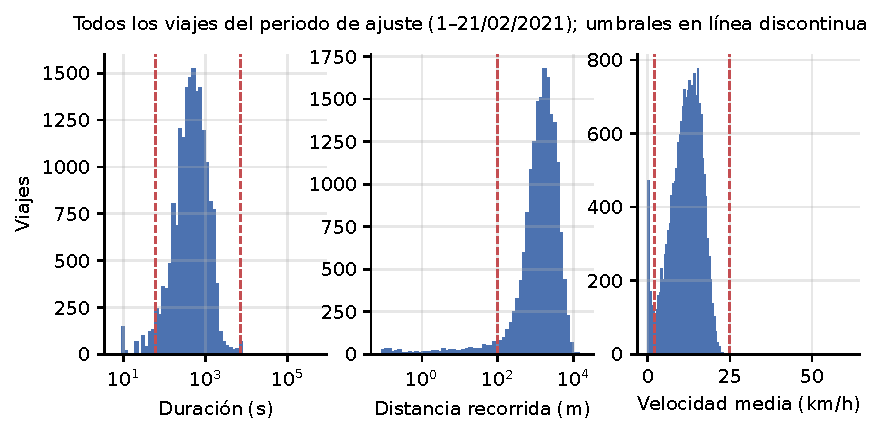
\includegraphics[width=\textwidth]{T10_umbrales}
  \caption{Histogramas de duración, distancia y velocidad con los umbrales de limpieza.}\label{fig:umbrales}
\end{figure}

% ------------------------------------------------------------------------------------------
\section{Exploración orientada a decisiones}

\subsection{El piloto recogía patinetes, no rebalanceaba en el día}
Al encadenar los viajes de cada patinete, el salto entre el final de uno y el inicio del
siguiente separa dos grupos: el ruido del GPS (mediana de \cifra{salto_mediana_m}~m) y
\cifra{recolocaciones} recolocaciones de más de 200~m, con una mediana de
\cifra{recolocacion_km}~km (\nb{exploracion/T11_recolocaciones.ipynb}). El patinete
recolocado ha estado parado una mediana de \cifra{parado_recolocado_h}~h, frente a
\cifra{parado_sin_salto_h}~h cuando no hay salto, y el \cifra{recolocaciones_noche_pct}\pc{}
de las recolocaciones incluye una noche. Son recogidas de varios días para cargar o reparar,
no rebalanceo dentro del día. Con estaciones de recarga esas recogidas desaparecen, y el
rebalanceo de la fase~1 se plantea nocturno.

\subsection{Patrones temporales}
En el ajuste hay \cifra{viajes_dia_ajuste} viajes al día. Laborables y fines de semana tienen
el mismo volumen (\cifra{viajes_dia_laborable} y \cifra{viajes_dia_finde}), pero no la misma
forma (figura~\ref{fig:calor}): el laborable tiene una punta de mañana de 7 a 10~h con el
\cifra{punta_manana_lab_pct}\pc{} de los viajes, frente al \cifra{punta_manana_finde_pct}\pc{}
del fin de semana, que concentra más en la tarde (\cifra{punta_tarde_finde_pct}\pc{} de 16 a
20~h). Por eso las matrices y el simulador separan los dos tipos de día y trabajan con cinco
franjas: madrugada (0--7), punta de mañana (7--10), mediodía (10--16), punta de tarde
(16--20) y noche (20--24) (\nb{exploracion/T12_temporal.ipynb}). Como mucho hay
\cifra{simultaneos_max} viajes en curso a la vez: es una cota muy floja de la flota, que
fijará la simulación de inventario por estación.

\begin{figure}[!htb]
  \centering
  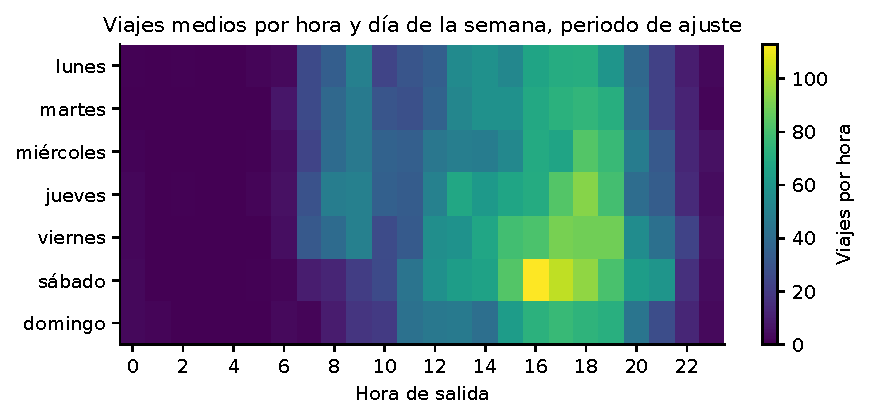
\includegraphics[width=0.9\textwidth]{T12_calor_dia_hora}
  \caption{Viajes medios por hora y día de la semana, periodo de ajuste.}\label{fig:calor}
\end{figure}

\subsection{La demanda en el espacio y la rejilla de candidatos}
Los orígenes y destinos se agregan en celdas hexagonales H3 \cite{h3}
(\nb{exploracion/T13_densidad.ipynb}). En resolución~8 (arista de \cifra{arista_res8_m}~m)
hay demanda en \cifra{celdas_res8} celdas; en resolución~9 (arista de
\cifra{arista_res9_m}~m, del orden del radio de acceso) en \cifra{celdas_res9}. La demanda
está repartida: el 20\pc{} de las celdas reúne el \cifra{concentracion_20pc_res8}\pc{} de los
extremos en resolución~8 (figura~\ref{fig:densidad}). Y es estable: la correlación de
Spearman de las cuotas por celda entre el ajuste y la semana reservada es
\cifra{estabilidad_res8} en resolución~8 y \cifra{estabilidad_res9} en resolución~9.
\textbf{Los candidatos a estación serán las celdas de resolución~9}; la resolución~8 queda
para mapas, saldos y matrices.

\begin{figure}[!htb]
  \centering
  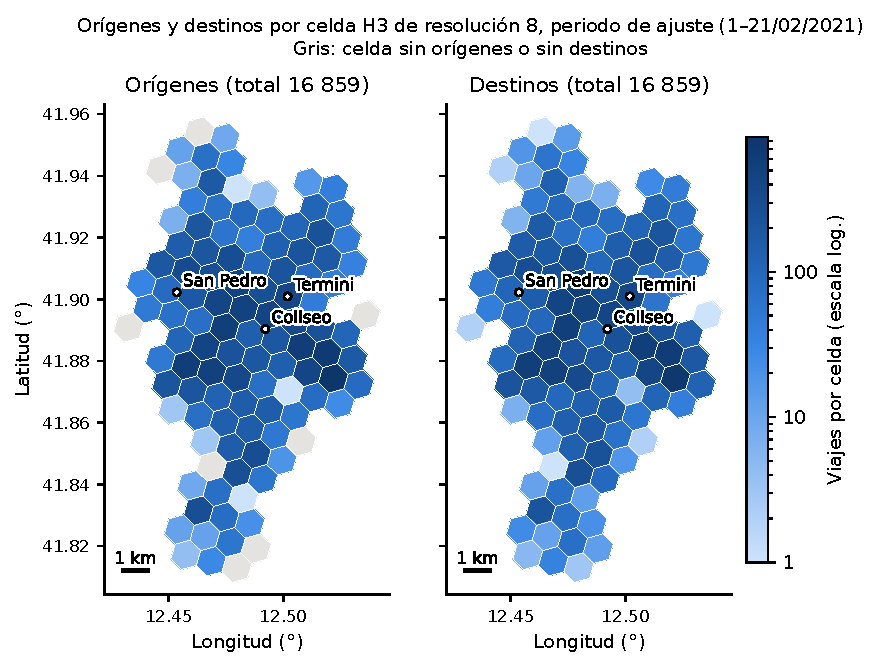
\includegraphics[width=0.75\textwidth]{T13_densidad_res8}
  \caption{Orígenes y destinos por celda H3 de resolución 8 en el periodo de ajuste.}\label{fig:densidad}
\end{figure}

\subsection{Saldo por celda y rebalanceo}
Si en una celda salen más viajes de los que llegan, se vacía; si llegan más, se llena
(\nb{exploracion/T14_saldo.ipynb}). De las \cifra{celdas_saldo} celdas con al menos 30
extremos, \cifra{celdas_emisoras} son emisoras y \cifra{celdas_receptoras} receptoras, y en
las que más desequilibrio tienen el saldo acumulado crece día tras día sin volver a cero.
Para devolver cada día cada celda a su estado inicial hay que mover al menos
\cifra{rebalanceo_res8} patinetes al día en resolución~8 y \cifra{rebalanceo_res9} en
resolución~9. El piloto ya lo hacía: las entregas netas del operador por celda siguen al
saldo de los viajes (Spearman de \cifra{operador_spearman}, figura~\ref{fig:operador}) y
compensan el \cifra{operador_compensado_pct}\pc{} del saldo. \textbf{El rebalanceo nocturno
forma parte del escenario base}, con \cifra{rebalanceo_base} patinetes al día.

\begin{figure}[!htb]
  \centering
  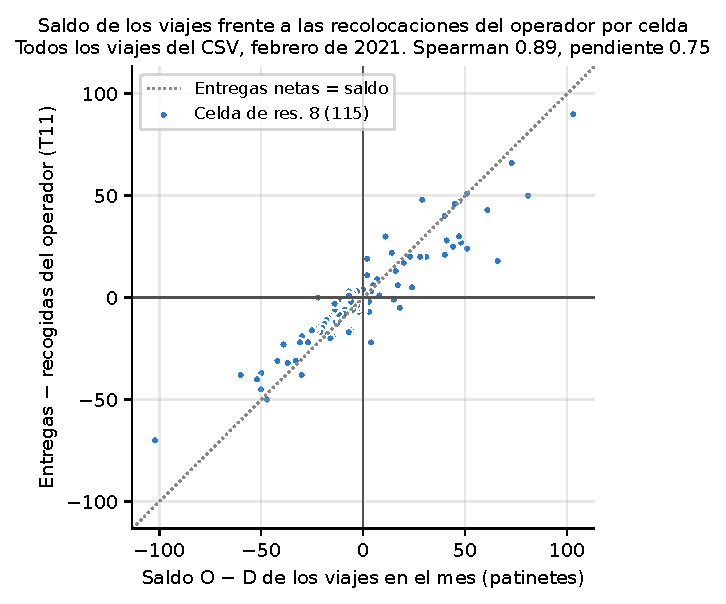
\includegraphics[width=0.62\textwidth]{T14_saldo_frente_operador}
  \caption{Entregas netas del operador frente al saldo de los viajes por celda de resolución 8, mes completo.}\label{fig:operador}
\end{figure}

\subsection{Recorridos y radios de acceso}\label{sec:radios}
El viaje mediano recorre \cifra{dis_mediana_m}~m en \cifra{tt_mediana_min}~min a
\cifra{vel_mediana}~km/h (\nb{exploracion/T15_recorridos.ipynb}). El recorrido es
\cifra{rodeo} veces la línea recta (mediana), y ese factor de rodeo pasa las distancias en
línea recta a distancias andando. Con estaciones, cada viaje paga el acceso a pie: si las
estaciones están a una distancia $R$ y se anda $2R/3$ en cada extremo, a
\cifra{velocidad_pie}~m/s \cite{bohannon2011}, andar a las estaciones tarda más que el propio
viaje en una parte creciente de los viajes (figura~\ref{fig:radios} y tabla~\ref{tab:radios}).
\textbf{Se barren radios de 200, 250 y 300~m y se deja 400~m como sensibilidad}. El
\cifra{circulares_pct}\pc{} de los viajes son circulares, así que el simulador admite origen
y destino en la misma estación.

\begin{figure}[!htb]
  \centering
  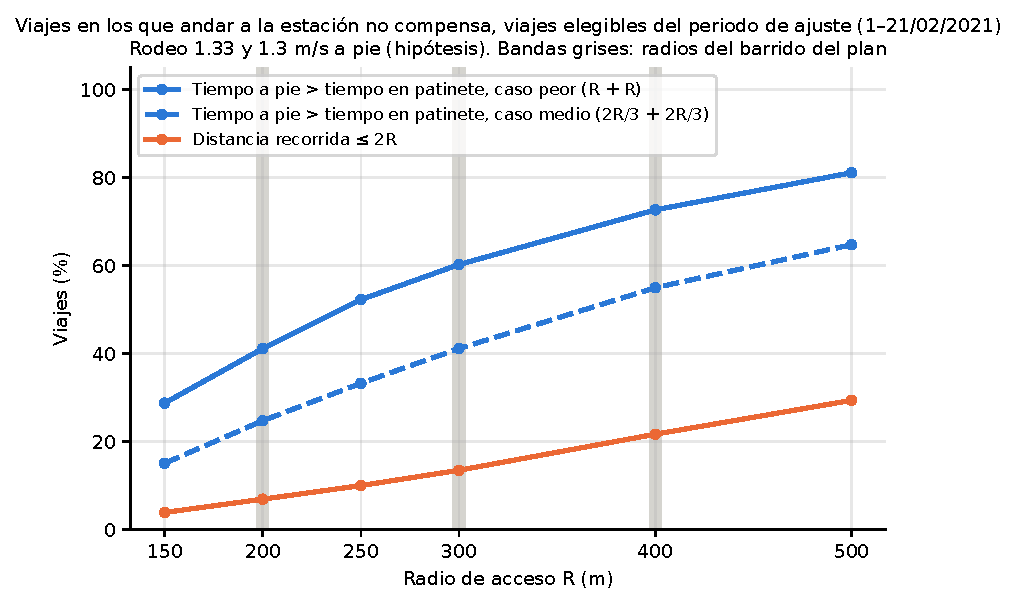
\includegraphics[width=0.72\textwidth]{T15_radios_acceso}
  \caption{Coste del acceso a pie según el radio de acceso, periodo de ajuste.}\label{fig:radios}
\end{figure}

La tabla~\ref{tab:radios} da además el orden de magnitud del número de estaciones: los
círculos de radio $R$ en malla hexagonal que cubren el área de las celdas de resolución~9 con
el 80 al 95\pc{} de los extremos. Es una cuenta de área, no una localización, y fija el rango
del barrido de la fase~1, ampliado un 20\pc{} por cada lado para que el óptimo no quede en el
borde.

\begin{table}[htb]
  \centering\small
  \caption{Radios de acceso: coste del acceso a pie (caso medio) y rango de estaciones del barrido.}\label{tab:radios}
  \begin{tabular}{@{}rlrrrr@{}}
    \toprule
    $R$ (m) & Papel & \makecell{Andar tarda más\\que el viaje (\%)} & \makecell{Viaje más corto\\que $2R$ (\%)} & \makecell{Estaciones\\(80--95\,\% de extremos)} & \makecell{Rango\\del barrido} \\
    \midrule
    % Generado por memoria/generar_cifras.py. No editar a mano.
200 & barrido & 24,9 & 6,6 & 230--387 & 184--465 \\
250 & barrido & 33,4 & 9,6 & 147--248 & 117--298 \\
300 & barrido & 41,3 & 13,1 & 102--172 & 81--207 \\
400 & sensibilidad & 55,2 & 21,2 & 58--97 & 46--117 \\
\bottomrule
% termina en \bottomrule
  \end{tabular}
\end{table}

\subsection{Meteorología: lluvia, viento y días anómalos}
La lluvia explica los días con pocos viajes (\nb{exploracion/T17_meteorologia.ipynb},
figura~\ref{fig:lluvia}). La correlación de Spearman de los viajes diarios con la lluvia es
\cifra{rho_lluvia}, y en las horas con lluvia hubo el \cifra{cociente_lluvia}\pc{} de los
viajes de la misma hora sin lluvia en los días de alrededor: el \cifra{cociente_lluvia_lab}\pc{}
en laborables y solo el \cifra{cociente_lluvia_finde}\pc{} en fin de semana. El único día por
debajo del 70\pc{} de la mediana de su tipo de día es el domingo 07/02 (\cifra{viajes_0702}
viajes, con \cifra{lluvia_0702}~mm). Es demanda real: no se excluye, pero no se usa como día
de diseño.

\begin{figure}[!htb]
  \centering
  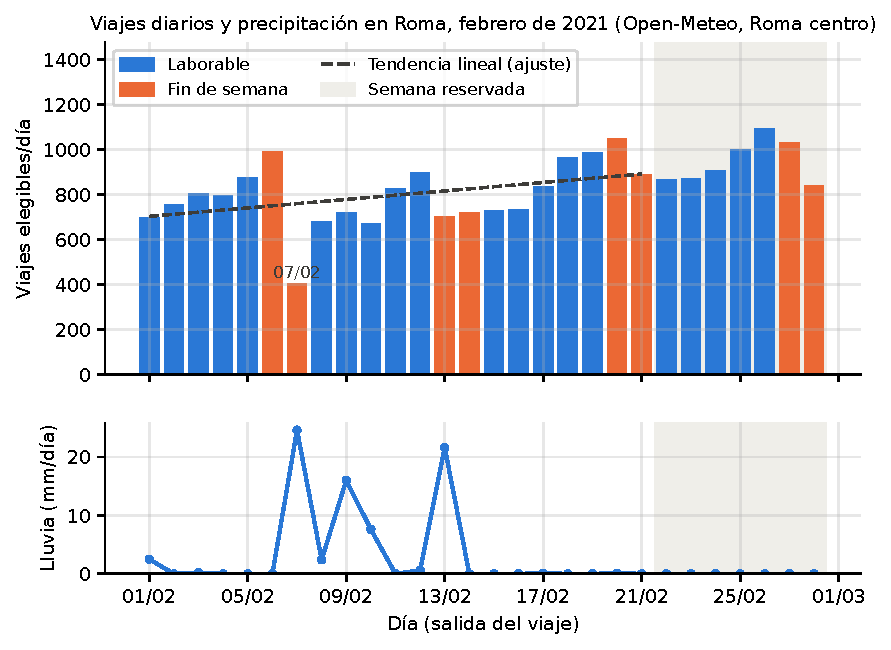
\includegraphics[width=0.78\textwidth]{T17_viajes_lluvia}
  \caption{Viajes diarios y precipitación. La zona sombreada es la semana reservada.}\label{fig:lluvia}
\end{figure}

En el fin de semana, el viento máximo se asocia con los viajes más que la lluvia
(\cifra{rho_viento_finde} frente a \cifra{rho_lluvia_finde}, con solo 8 días), y había que
saber si era el mismo efecto. No lo es (figura~\ref{fig:viento}). Viento y lluvia apenas van
juntos (\cifra{rho_viento_lluvia_finde}), y descontando la lluvia la correlación del viento
sigue en \cifra{rho_viento_parcial_finde}. Por horas, con lluvia, viento, temperatura y
tendencia en el mismo modelo, 10~km/h más de viento quitan un \cifra{viento_finde_pct}\pc{}
de los viajes del fin de semana (intervalo al 95\pc{} de \cifra{viento_finde_inf} a
\cifra{viento_finde_sup}\pc{}) y solo un \cifra{viento_lab_pct}\pc{} en laborables, sin
diferencia clara con cero. La prueba descansa en un episodio: el fin de semana frío y
ventoso del 13--14/02 (el 14/02, sin lluvia, tuvo \cifra{viajes_1402} viajes). \textbf{El
viento fuerte reduce por sí mismo la demanda de ocio del fin de semana, menos que la lluvia,
y casi no afecta a los laborables.} No entra en el simulador; el 13 y el 14/02 se tratan como
el 07/02.

\begin{figure}[!htb]
  \centering
  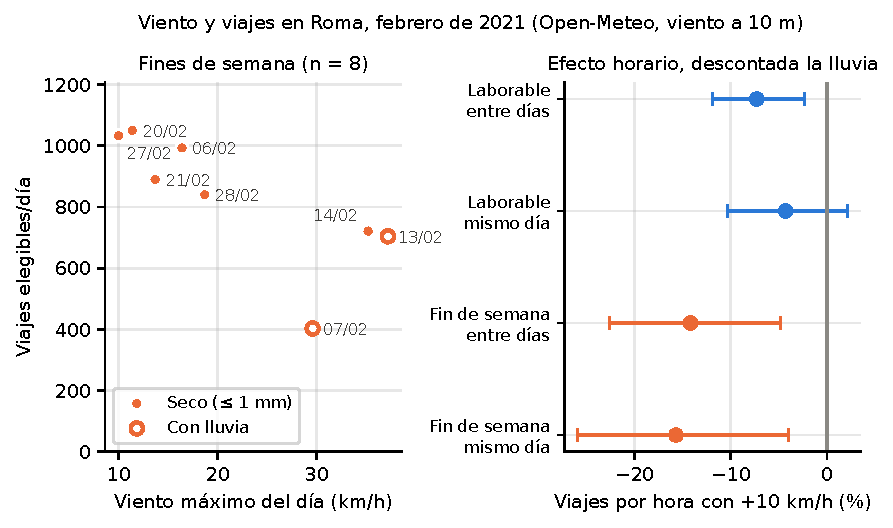
\includegraphics[width=0.85\textwidth]{T17_viento}
  \caption{Viento y viajes. Izquierda: los 8 días de fin de semana (huecos, con lluvia). Derecha: efecto horario de 10~km/h más de viento descontada la lluvia, con su intervalo al 95\,\%.}\label{fig:viento}
\end{figure}

La semana reservada tiene un \cifra{reservada_mas_pct}\pc{} más de viajes al día que el
ajuste. No llovió, fue más cálida (\cifra{temp_reservada} frente a \cifra{temp_ajuste}~°C)
y tuvo menos viento. Al tener en cuenta la lluvia y la temperatura, la pendiente de los
viajes en el mes baja de \cifra{pendiente_mes} a \cifra{pendiente_mes_tiempo} viajes al día
por cada día, pero no desaparece: el tiempo explica parte del crecimiento, no todo. La
validación con la semana reservada es, por tanto, más exigente que el ajuste. Se validarán
las cuotas (reparto de viajes entre estaciones, pares y franjas), que no dependen del
volumen, y la diferencia de volumen se presentará como resultado.

% ------------------------------------------------------------------------------------------
\section{Movilidad}

\subsection{Primera matriz origen-destino}
Con las celdas de resolución~8, los viajes del ajuste se reparten en \cifra{od_pares} pares
origen-destino (\nb{movilidad/T20_matrices_od.ipynb}, figura~\ref{fig:od}). El
\cifra{od_intrazonales_pct}\pc{} no sale de su celda, los 20 pares más frecuentes suman el
\cifra{od_top20_pct}\pc{} y las 30 celdas con más extremos reúnen el \cifra{od_top30_pct}\pc{}
de los viajes. Cada par es casi simétrico: la asimetría observada es \cifra{od_asimetria}
veces la esperable por azar. No hay corredores de ida sin vuelta; el saldo de cada celda es
la suma de muchos pares pequeños, y el rebalanceo se plantea por zonas.

\begin{figure}[!htb]
  \centering
  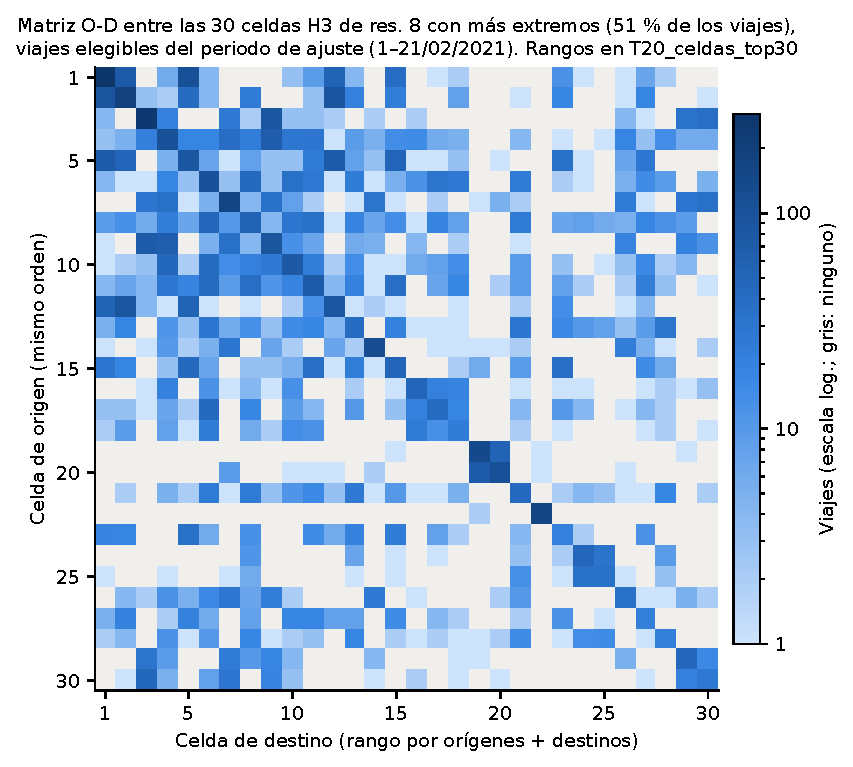
\includegraphics[width=0.62\textwidth]{T20_od_top30}
  \caption{Matriz origen-destino entre las 30 celdas de resolución 8 con más extremos (escala logarítmica), periodo de ajuste.}\label{fig:od}
\end{figure}

\subsection{Método previsto para la red}
\begin{enumerate}
  \item Matrices por franja horaria y tipo de día, y por zonas administrativas.
  \item Candidatos: centros de las celdas de resolución~9 con demanda.
  \item Localización con el mismo conjunto de candidatos y viajes: K-medoids como línea base,
        cobertura de conjuntos (LSCP), $p$-mediana y cobertura máxima (MCLP), con $k$ en el
        rango de la tabla~\ref{tab:radios} para cada radio. El frente de Pareto entre número
        de estaciones y distancia a pie en origen y destino da la red elegida.
  \item Asignación de cada viaje a sus estaciones y simulación de inventario por franjas, con
        rebalanceo nocturno de \cifra{rebalanceo_base} patinetes al día (\cifra{rebalanceo_sensibilidad} como sensibilidad), para fijar
        los anclajes y los patinetes de cada estación y la curva de flota frente a nivel de
        servicio.
  \item Validación con la semana reservada.
\end{enumerate}

% ------------------------------------------------------------------------------------------
\section{Consumo}
Con el consumo medio del enunciado, 13,5~Wh/km, y la batería de 576~Wh, la flota observada
gasta \cifra{flota_kwh_dia}~kWh al día en el ajuste, con un máximo de
\cifra{flota_kwh_dia_max} (\cifra{flota_cargas_dia} cargas completas al día de media;
\nb{exploracion/T16_energia_referencia.ipynb}). Ningún viaje ni ningún patinete en un día
llega a gastar la batería entera, y la autonomía mediana con el uso observado es de
\cifra{autonomia_mediana_dias} días: con esta flota, cada patinete se recargaría cada varios
días. Es una referencia. Con estaciones y una flota simulada menor, cada patinete hará más
viajes, así que el consumo por patinete y por estación se calculará con la flota de la
simulación.

Método previsto: modelo A con 13,5~Wh/km por viaje; modelo B físico con rodadura,
aerodinámica, pendiente (desnivel origen-destino) y aceleración, calibrado frente a 13,5~Wh/km;
consumo por viaje, patinete, flota y estación; y estado de carga de cada patinete a lo largo
del mes.

% ------------------------------------------------------------------------------------------
\section{Estación de recarga}
La exploración fija la escala de una estación: la celda de resolución~8 que más energía
recibe llega a \cifra{celda_kwh_max}~kWh al día, y la mediana es de \cifra{celda_kwh_p50}.
Una estación cubrirá menos área que una de esas celdas, así que su demanda será de décimas de
kWh a 1~kWh al día. La energía llega sobre todo sin sol (figura~\ref{fig:perfil}): solo el
\cifra{energia_sol_pct}\pc{} de los viajes acaba de 10 a 16~h, y el \cifra{energia_tarde_pct}\pc{}
de 16 a 24~h. Si se carga en cuanto llega el patinete, la batería de la estación debe guardar
unos dos tercios de la energía; retrasar la carga a las horas de sol es la alternativa.

\begin{figure}[!htb]
  \centering
  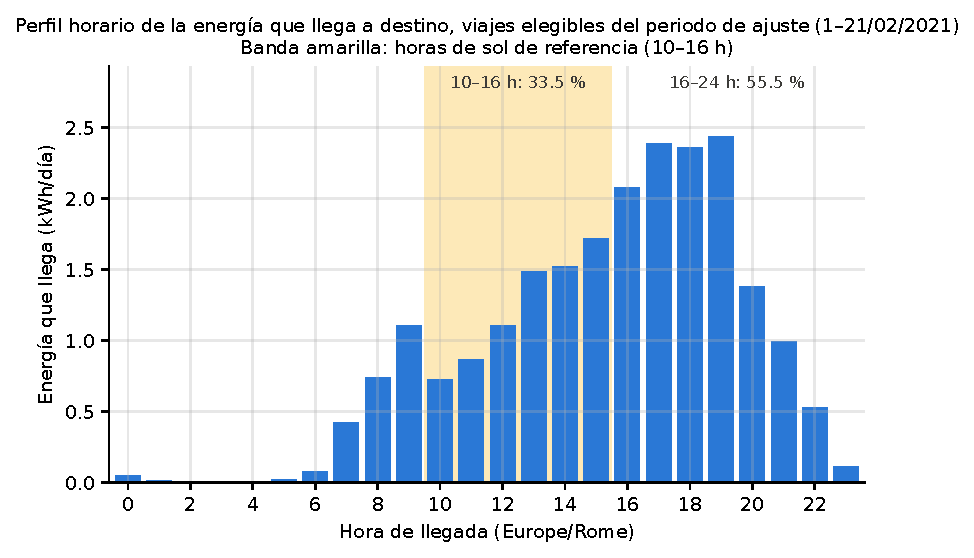
\includegraphics[width=0.7\textwidth]{T16_perfil_horario}
  \caption{Energía que llega por hora del día (consumo de los viajes que acaban en esa hora), periodo de ajuste.}\label{fig:perfil}
\end{figure}

Método previsto: curvas de potencia y energía de todas las estaciones; elección de la
estación concreta; producción fotovoltaica horaria con PVWatts \cite{pvwatts}; balance horario
de paneles, batería (4, 8 o 12~kWh) y red; y barrido de paneles por batería hasta que la
estación sea autónoma la mayor parte del tiempo.

% ------------------------------------------------------------------------------------------
\section{Conclusiones provisionales y limitaciones}

\begin{table}[H]
  \centering\small
  \caption{Decisiones de la fase 0 que usan las fases siguientes (detalle en \texttt{docs/conclusiones\_eda.md} \cite{codigo}).}\label{tab:decisiones}
  \begin{tabularx}{\textwidth}{@{}lY@{}}
    \toprule
    Decisión & Valor \\
    \midrule
    Viajes elegibles & \cifra{viajes_elegibles}: umbrales de 60~s, 100~m, 2~km/h, 25~km/h y 2~h \\
    Periodos & Ajuste del 1 al 21/02; validación con la semana del 22 al 28/02 \\
    Franjas y tipos de día & Cinco franjas; laborable y fin de semana por separado \\
    Rejilla & Candidatos en H3 de resolución~9; mapas y matrices en resolución~8 \\
    Radios de acceso & 200, 250 y 300~m; 400~m como sensibilidad; rodeo de \cifra{rodeo} y \cifra{velocidad_pie}~m/s a pie \\
    Número de estaciones & Rango del barrido de la tabla~\ref{tab:radios} para cada radio \\
    Rebalanceo & Nocturno, \cifra{rebalanceo_base} patinetes al día en el escenario base; \cifra{rebalanceo_sensibilidad} como sensibilidad \\
    Días de diseño & Ninguno se excluye; el 07/02 (lluvia) y el 13--14/02 (viento fuerte y frío) no son días de diseño \\
    Energía de referencia & \cifra{flota_kwh_dia}~kWh al día para la flota observada; décimas de kWh a 1~kWh al día por estación \\
    \bottomrule
  \end{tabularx}
\end{table}

Las decisiones de la tabla~\ref{tab:decisiones} están en \nb{config.yaml} y las leen todas
las tareas. Limitaciones conocidas hasta ahora:
\begin{itemize}
  \item Sin trayectorias: las distancias a pie se estiman con el factor de rodeo del patinete
        y una velocidad a pie supuesta; se contrastarán con la red peatonal en las redes
        finalistas.
  \item Un solo mes de invierno, con crecimiento dentro del mes y una semana de validación más
        cálida, seca y con más demanda.
  \item La demanda observada es la de un servicio sin estaciones; parte de ella no tendría
        sentido con estaciones (el \cifra{circulares_pct}\pc{} son viajes circulares y, con
        300~m, andar a las estaciones tarda más que el viaje en cuatro de cada diez).
  \item No se ha podido leer el texto oficial de las restricciones por COVID en Lacio en
        febrero de 2021, así que no se controla el contexto sanitario del mes.
\end{itemize}

\printbibliography[heading=bibintoc,title={Referencias}]

\end{document}
